% !TeX root = ../main.tex
\chapter{背景介绍}
\label{chap:background}
\section{环境反向散射通信}
\begin{figure}
	\centering
	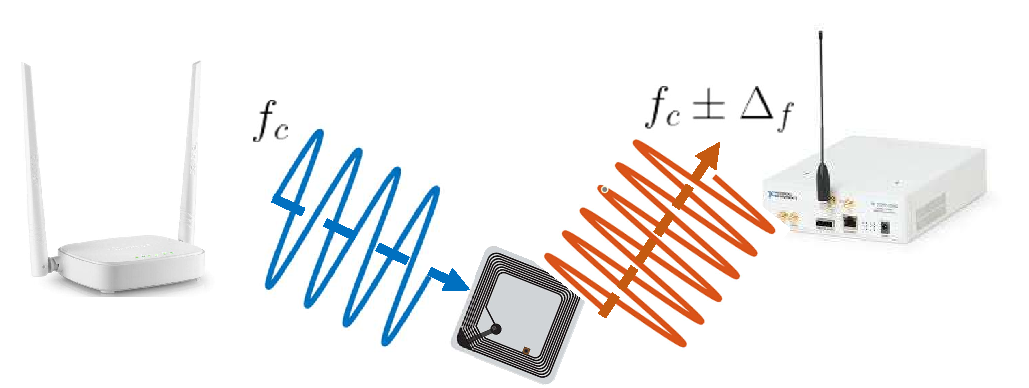
\includegraphics[width = .7\linewidth]{bkg_figure1_system-cropped}
	\caption{环境反向散射通信系统构成。标签(中间)会对环境中的信号进行调制。}
	\label{fig:system}
\end{figure}
环境反向散射通信可以视为以RFID为代表的传统反向散射通信方法的一个延伸。一个反向散射通信系统由三部分组成:激励源,反向散射标签和接收器。对于传统的反向散射通信,激励源是一个预设好的设备,会发射特定的电磁波信号;而环境反向散射通信利用环境中已经存在的电磁信号,如电视和广播等,获取能量并对已存在的电磁信号进行调制完成通信。图\ref{fig:system}展示了一个典型的利用Wi-Fi信号进行反向散射通信的系统。Wi-Fi AP在正常传输数据,反向散射标签对原始的进行调制,将自身要传输的信息添加在原始信号中,接收端对调制后的信号进行监听,从中完成解码。

反向散射标签通过改变天线的阻抗实现对已有信号的调制。当电磁波遇到具有不同阻抗的介质交界面时,部分电磁波会被反射回来;而天线的阻抗与周围环境的阻抗不同,因此会有部分信号被天线反射。通过调整天线的阻抗即可实现对反射回的电磁波能量的控制。当入射信号为$S_{in}$时,被反射回的信号$S_{out}$可以表示为:
\begin{equation}
S_{out} = S_{in} \frac{Z_a - Z_c}{Z_a + Z_c},
\end{equation}
其中$Z_a$是天线阻抗,$Z_c$是与天线相连的电路阻抗。通过将天线短接与否可以控制反射信号的能量大小:短接时反射全部信号,不断接时吸收信号。这两种状态的变化可以用来传递比特1和0。这种调制方案在反向散射通信中广泛使用,成为开关键控(On-off keying, OOK)。假设背景流量的信号工作在$f_c$频率上,OOK可以看作对使用一个频率为$\Delta f$的方波$S$与背景信号相乘。在近似的情况下,采用方波的傅里叶分解的基波成分,有下式成立:
\begin{equation}
\begin{split}
	\sin(2\pi f_c t)\cdot S &\approx \sin(2\pi f_c t)\cdot \sin(2\pi \Delta_f t)\\
	& =\frac{\cos (2\pi (f_c - \Delta_f)t) - \cos (2\pi (f_c + \Delta_f)t)}{2}.
\end{split}
\end{equation}
因此,原始信号被OOK调制偏移到频率$f_c \pm \Delta_f$上,以减轻与原始信号之间的干扰。

\section{里德-所罗门码与突发错误}
\begin{figure}
	\centering
	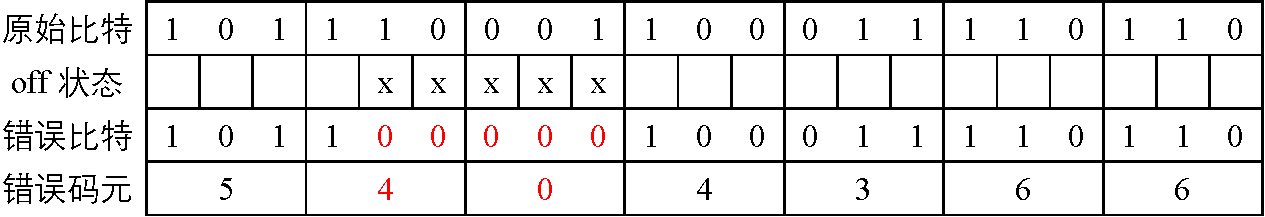
\includegraphics[width = \linewidth]{bkg_figure2_RSburst-cropped}
	\caption{里德-所罗门码将突发错误转变成数量更少的码元错误,从而在恢复突发错误上具有优势。}
	\label{fig:rscode}
\end{figure}
里德-所罗门码是一种前向错误更正编码,被广泛地应用于CD、DVD 和蓝光光盘上以及广播系统中 DVB标准中。 
一个里德-所罗门码$RS_{n,k}$是一种定义在有限域$\symup{F}$上的长度为$n$,信息长度为$k$,最短汉明距离为$n-k+1$的线性分组码;在实际应用中,有限域$\symup{F}$通常指定为$\symup{GF}(2^m)$,在这种情况下,每个码元都包含有$m$比特的信息。

$RS_{n,k}$码非常适合纠正传输系统中的突发错误。以图\ref{fig:rscode}为例,假设当前环境中的Wi-Fi流量的ON/OFF状态如第二行所示,其中标x的部分表示当现有OFF状态。
如果我们使用$RS_{7,3}$码进行编码,那么每3个比特构成一个码元,如第四行所示。尽管在比特上存在5个突发错误,但是在码元的角度来看只有2个码元发生了错误,因此$RS_{7,3}$可以正确将该突发错误恢复。
也即,不论一个码元中有多少个比特发生错误,都只发生了一个码元错误;因此里德-所罗门码适合纠正传输系统中的突发错误,也因此适用于反向散射通信中Wi-Fi空闲状态造成的错误纠正。
\section{低密度奇偶校验码}

LDPC编码是一种接近信道容量的编码,在合适的构造情况下性能可以接近香农限。1963年,Gallager首次提出了LDPC码,但在当时由于实现上的困难一直没有得到重视。在1996年,Mackay等人对LDPC码进行了重新的发现,自此该码收到更多的关注和发展。

LDPC码是基于具有稀疏矩阵性质的奇偶检验矩阵$H$建构而成。按照奇偶检验矩阵,LDPC码可分为规则和非规则
两种。规则 LDPC 码中,各行1的个数(称为行重)相同且各列1的个数(称为列重)相同。而行重或者列重不一致就称为非规则LDPC码。
每一行可以代表一个对所有比特的校验,因此行重一致表示每个检验由相同个数的比特参与;而列重一致表明每个比特参与的校验个数是相同的。$H$的结构中就包含了交织特性。
